
\setlength{\abovedisplayskip}{5pt}
\setlength{\belowdisplayskip}{5pt}

\rightline{(文責:アメリカムシクイ)}

\subsection{はじめに}
\begin{multicols}{2}
ボードゲームは、麻雀と並ぶ寮内娯楽の一つである。麻雀は年に2度全寮的な麻雀大会が開かれるほどには寮生の間に浸透しており、どの談話室でも遊ばれている。一方でボードゲームは麻雀ほどメジャーな遊びではないものの、ボドゲ新歓という食堂でボードゲームを遊ぶ交流会が開かれる程度には人気な娯楽だ。寮でよく遊ばれるボードゲームは、カタンやとドミニオンでろう\footnote{中でもカタンは私が一番好きなボドゲだ。寮祭で耐久カタンという企画が開かれるほどには人気で、\sout{正直ウィングスパンをしながら「こんなことやってないでカタンの研究がしたい」といつも思っている。}一方でウィングスパンはどちらかというとマイナーで、私が存在を確認している談話室は3か所しかない。そのうち1つは私がこの記事の原稿を書き終えた後に布教した。}。この2つは寮のどこの談話室に行っても大抵置いてある。そして、本記事で扱うWINGSPAN(ウィングスパンと読む。)も数多あるボードゲームの一つだ。
\par
先日(と言ってもこの入寮パンフレットができあがるころには1年近く経ってしまっているが)、知り合いの寮生たちの間で開いた耐久ボドゲ会\footnote{一日中ボドゲをして遊ぶという尊くて幸せな会。私がよく主催して、知り合いのボドゲ好きな寮生たちと遊んでいる。通常「耐久する」という言葉は、夜通し何か一つのことをして徹夜するという行為をさす。例えば耐久麻雀と言えば、徹夜で麻雀をするという意味である。ただ徹夜をするのは身体が耐えられないので、夜の代わりに昼間に遊んでいる。}で、ウィングスパンを遊ぶ機会があった。第2章で述べるようにウィングスパンは各プレイヤーが鳥の生態系を作るゲームであるが、私は以前から、こうした自分の世界で拡大再生産するタイプのボドゲがあまり得意ではなかった。たいていこの種のボドゲはAを作るのにBが必要で、Bを作るのにCが必要で、Cを作るのにAが必要、といった具合に、ゲームで必要になるものを作るための手段が巡り巡ってループしており、序盤に何をすべきかがいつも分からないからだ。その会でもコツが掴めないままゲームが終わってしまったが、ゲーム自体は参加者に好評であった。せっかくみんなが好きになってくれたならと、苦手克服のために研究を始めることにした。
\par
ウィングスパンの苦手なところは序盤に何をすべきか分からない、ということであったから、始めた当初は序盤の定石を明らかにしたら終わりにしようと思っていた。しかし、研究を進めるにつれて、初めに想像していたよりも定石の分岐が複雑だということが分かり、より深く調べるために鳥カードの分類を始めてしまった。しまいには談話室の雑記帳の半分近くが研究の進捗で埋まり、ウィングスパンにある170羽の鳥の分類表を完成させるに至っていた。廃人になるまで1か月もかからなかった。
\par
あまりにも成果が多かったことと、談話室の雑記帳にとどめておくだけではもったいないと思ったことから、今回入寮パンフの記事として書くことにした。寮内のプレイヤーが少ないボドゲの考察記事を書いたところで喜ぶ人がどれくらいいるかは分からないが、この記事が寮のボドゲ文化のさらなる盛り上がりに寄与したらとてもうれしい限りである。
\par
次章に入る前に、本記事の構成を述べる。最初にウィングスパンの概要としてルール、得点方法について述べる。その後これらの情報から理想的な立ち回りを一つ提示し、その立ち回りがうまくいかない場合を例外として整理する。最後に個々の例外に対して対処法を与え、理想的な立ち回りの一例を完成させる。なお、ウィングスパンには拡張版がいくつかあるが、本記事で考察するのは無印のものに限ること、加えて研究はオートマ戦(一人プレイ)をもとにしたことをここで言及しておく。
\end{multicols}
\subsection{WINGSPANの概要}
\begin{multicols}{2}
\subsubsection{ルールの概要}
考察に入る前に、ウィングスパンのルールについて概説する。ルールをご存じの方は飛ばしてもらって構わない。
\par
ウィングスパンは各プレイヤーに配られたゲームボードに鳥カードや卵を配置していって、プレイヤーごとに生態系を作っていくゲームである。4ラウンド合計26ターンをかけて生態系を作り、ボード上の様々な要素に対して与えられた得点の合計を計算して、最も多くの得点を得たプレイヤーが勝者となる。基本は2~5人で遊ぶものだが、1人で遊ぶためのルールもあり、私のような独り者にも優しいボードゲームとなっている。
\par
ゲームが始まる前に各プレイヤーは5枚の鳥カードと2枚のボーナスカードが配られる。鳥カードは鳥の絵柄が書かれたカード、ボーナスカードは鳥カードに関する条件が書かれたカードで、その条件の達成度合いに応じてゲーム終了時に点数が得られる。プレイヤーはそのうち鳥カードを好きな枚数捨て、捨てた数と同じ種類だけ餌トークンを1個ずつ得る。そして2枚のボーナスカードのうち1枚を選び、選ばなかった方を捨てなければならない。ここまでが最初の準備である。
\par
各プレイヤーが最初の準備を終えた後は、プレイする順番を決め、1ラウンドの1ターン目からゲームが始まる。そのターンですべてのプレイヤーがプレイしたら、今度は1ラウンドの2ターン目になり、また1ターン目と同じ順番でプレイしていく。ラウンドが変わるごとに最初にプレイする人を変えながら、26回これを繰り返す\footnote{1ラウンド目は8ターン、2ラウンド目は7ターン、というようにラウンドが1つ進むごとにそのラウンドでのターン数は1つずつ減少していく。}。また、ラウンドごとにラウンド終了時目的というものがランダムに決められており、その達成度合いによりプレイヤーごとに点数が配分される。そのため、各プレイヤーはラウンドごとのラウンド終了時目的を達成できるように、さらにゲーム全体を通してボーナスカードの条件をできる限り達成できるように、プレイすることとなる。
\par
各ターンでプレイヤーができることは鳥カードのプレイ、餌の獲得、産卵、鳥カードの獲得、の4つのうちどれか1つである。ターンごとに、手元にある色つきの小さな立方体をしたことの目印として置いていくと、残りのターン数やそのラウンドでの行動が分かって親切だ。
\par
鳥カードのプレイを選択すると、自分の手札の中から1枚選んでボードに置くことができる。置く場所は、ボード上の空いている四角のマスのうち、各行で最も左側にあるマスのどこかである(図\ref{fig:実際にプレイしている様子}を参照)。ただし、どの行にも置いていいわけではなく、鳥カードの左上に書かれた生息地と同じ生息地の行にしか置けない。また置く際はプレイした鳥カードに書かれた餌と、置いたマスの列の一番上に書かれている卵の絵柄の数だけボード上にある卵を捨てなければならない。餌が足りない、あるいは卵を十分に捨てられない場合は、鳥カードをプレイすることはできない。プレイした鳥カードがプレイ時能力を持っているときは、その能力を発動させることができる\footnote{ウィングスパンのルールにおいて「~することができる」という表現が付くときは、それをしてもいいししなくてもいい、という意味である。例えばこの時は、プレイ時能力を発動させてもいいし、させない選択肢をとることもできる。以下、同じような表現をこの意味で用いる。}。
\begin{figure*}[htbp]
   \centering
   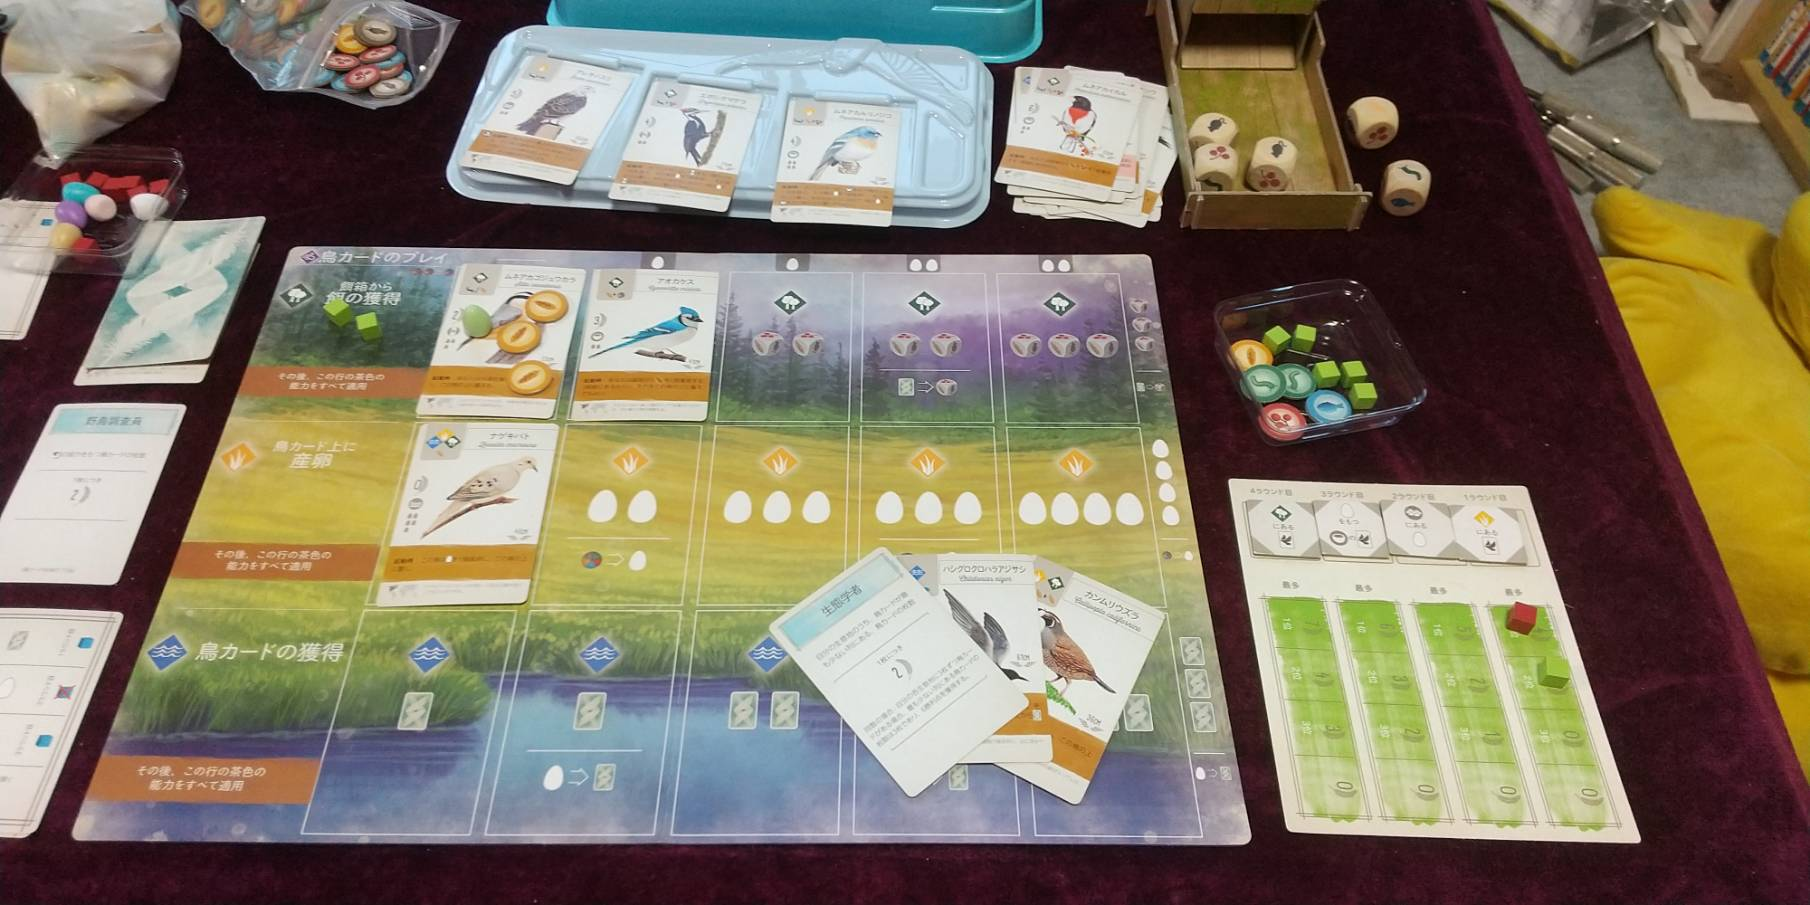
\includegraphics[height=7cm,width=15cm]{2025shinki/wing_span/real_play.jpg}
   \caption{実際にプレイしている様子}
   \label{fig:実際にプレイしている様子}
\end{figure*}
\par
餌の獲得を選択すると、一番上の行(森林)の空いているマスのうち最も左側に描かれたダイスの絵の数だけ餌トークンを獲得することができる。その際は、紙でできた餌箱の中にあるダイスを獲得する餌の数だけ外に移し、そのダイスの目が示している種類の餌を獲得する。餌箱からダイスがなくなった、あるいは餌箱にあるダイスの目がすべて同じときは、獲得する前にダイスをすべて振りなおすことができる。餌を獲得した後は、森林にプレイされている鳥カードの起動時能力を右端から順に発動させることができる。
\par
産卵を選択すると、二番目の行(草原)の空いているマスのうち最も左に描かれた卵の数だけ卵トークンを獲得し、プレイされている鳥カードが生むことができる卵の数を超えないように、好きな鳥カードの上に卵を置いていくことができる。産卵した後は、餌の獲得の時と同様に、草原にプレイされている鳥カードの起動時能力を右端から順に発動させることができる。
\par
鳥カードの獲得を選択すると、一番下の行(水辺)の空いているマスのうち最も左側に描かれた鳥カードの数だけ鳥カードを獲得することができる。この際、鳥カードは公開されている3枚の中から引くか、非公開にされている鳥の山の上から引くかを一枚ごとに選択することができる。公開されている3枚の中から引いた場合、引かれた分をトレイに補充するのはそのプレイヤーのターンが終わったときである。鳥カードを引いた後は、他の2つと同様に、水辺にプレイされている鳥カードの起動時能力を右端から順に発動させることができる。
\par
このようにゲームが進行していき、最終的には各プレイヤーごとに点数を計算していく。計算方法は、プレイされている鳥カードの得点の合計、ボーナスカードで得られた点数、ラウンド終了時目的から得られた点数、鳥カード上に産卵されている卵の総数、鳥カードの上に蓄えられている餌の総数、鳥カードに差し込まれている鳥カードの総数、の6項目の総和である。この総和が各プレイヤーの最終的な得点となり、その得点が大きい順に順位が決定していく。
\subsubsection{得点方法の分析}
ボードゲームの考察を行う際に最初にすべきことは、得点方法を整理することである。ウィングスパンにおいて、点数は以下の方法で得られる。
\begin{itemize}
  \item プレイした鳥カード
  \item ボーナスカード
  \item ラウンド終了時目的
  \item 卵
  \item 鳥の上に蓄えた餌
  \item 差し込んだ鳥カード
\end{itemize}
見方を変えれば、ウィングスパンはこの6通りの方法で得られた点数を競うゲームと言える。それぞれの項目で点数を増やすにはどうすればいいかを列挙すると、
\begin{itemize}
  \item プレイした鳥カード:鳥をたくさんプレイする。プレイするには「鳥カードを獲得→餌を獲得→(必要に応じて卵を獲得)→プレイ」
  という手順を踏む。
  \item ボーナスカード:条件を満たしている鳥をたくさんプレイする。
  \item ラウンド終了時目的:鳥をたくさんプレイするか、卵をたくさん産む。
  \item 卵:卵をたくさん産む。
  \item 鳥の上に蓄えた餌:鳥の能力をたくさん使う(やや特殊)
  \item 差し込んだ鳥カード:鳥の能力をたくさん使う(やや特殊)
\end{itemize}
という感じになる。基本的にはすべて鳥カードのプレイか産卵で賄えることが分かる。以上の得点方法と餌の獲得、鳥カードの獲得をまとめて、発展\footnote{本記事では、各生息地に鳥カードをプレイすることを、その生息地を「発展させる」と表現することがよくある。}の構造を図にすると図\ref{fig:発展構造}のようになる。
\begin{figure*}[htbp]
\begin{minipage}[b]{.5\textwidth}
  \centering
  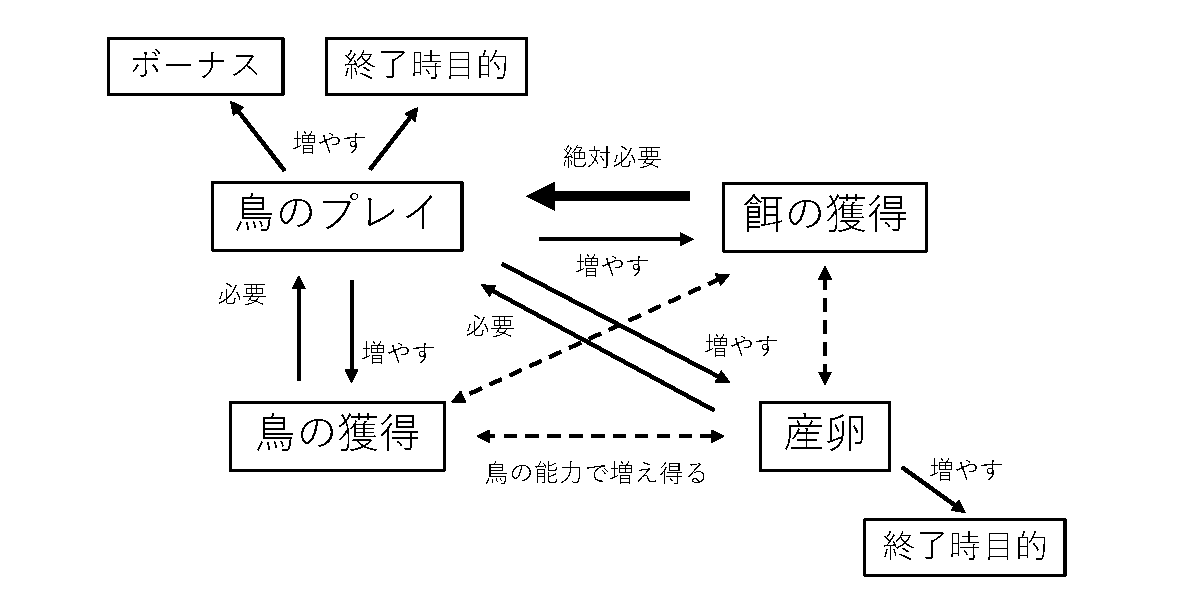
\includegraphics[height=4.2cm,width=8cm]{2025shinki/wing_span/WS_hattenkouzou.pdf}
  \caption{発展構造}
  \label{fig:発展構造}
\end{minipage}
\begin{minipage}[b]{.5\textwidth}
  \centering
  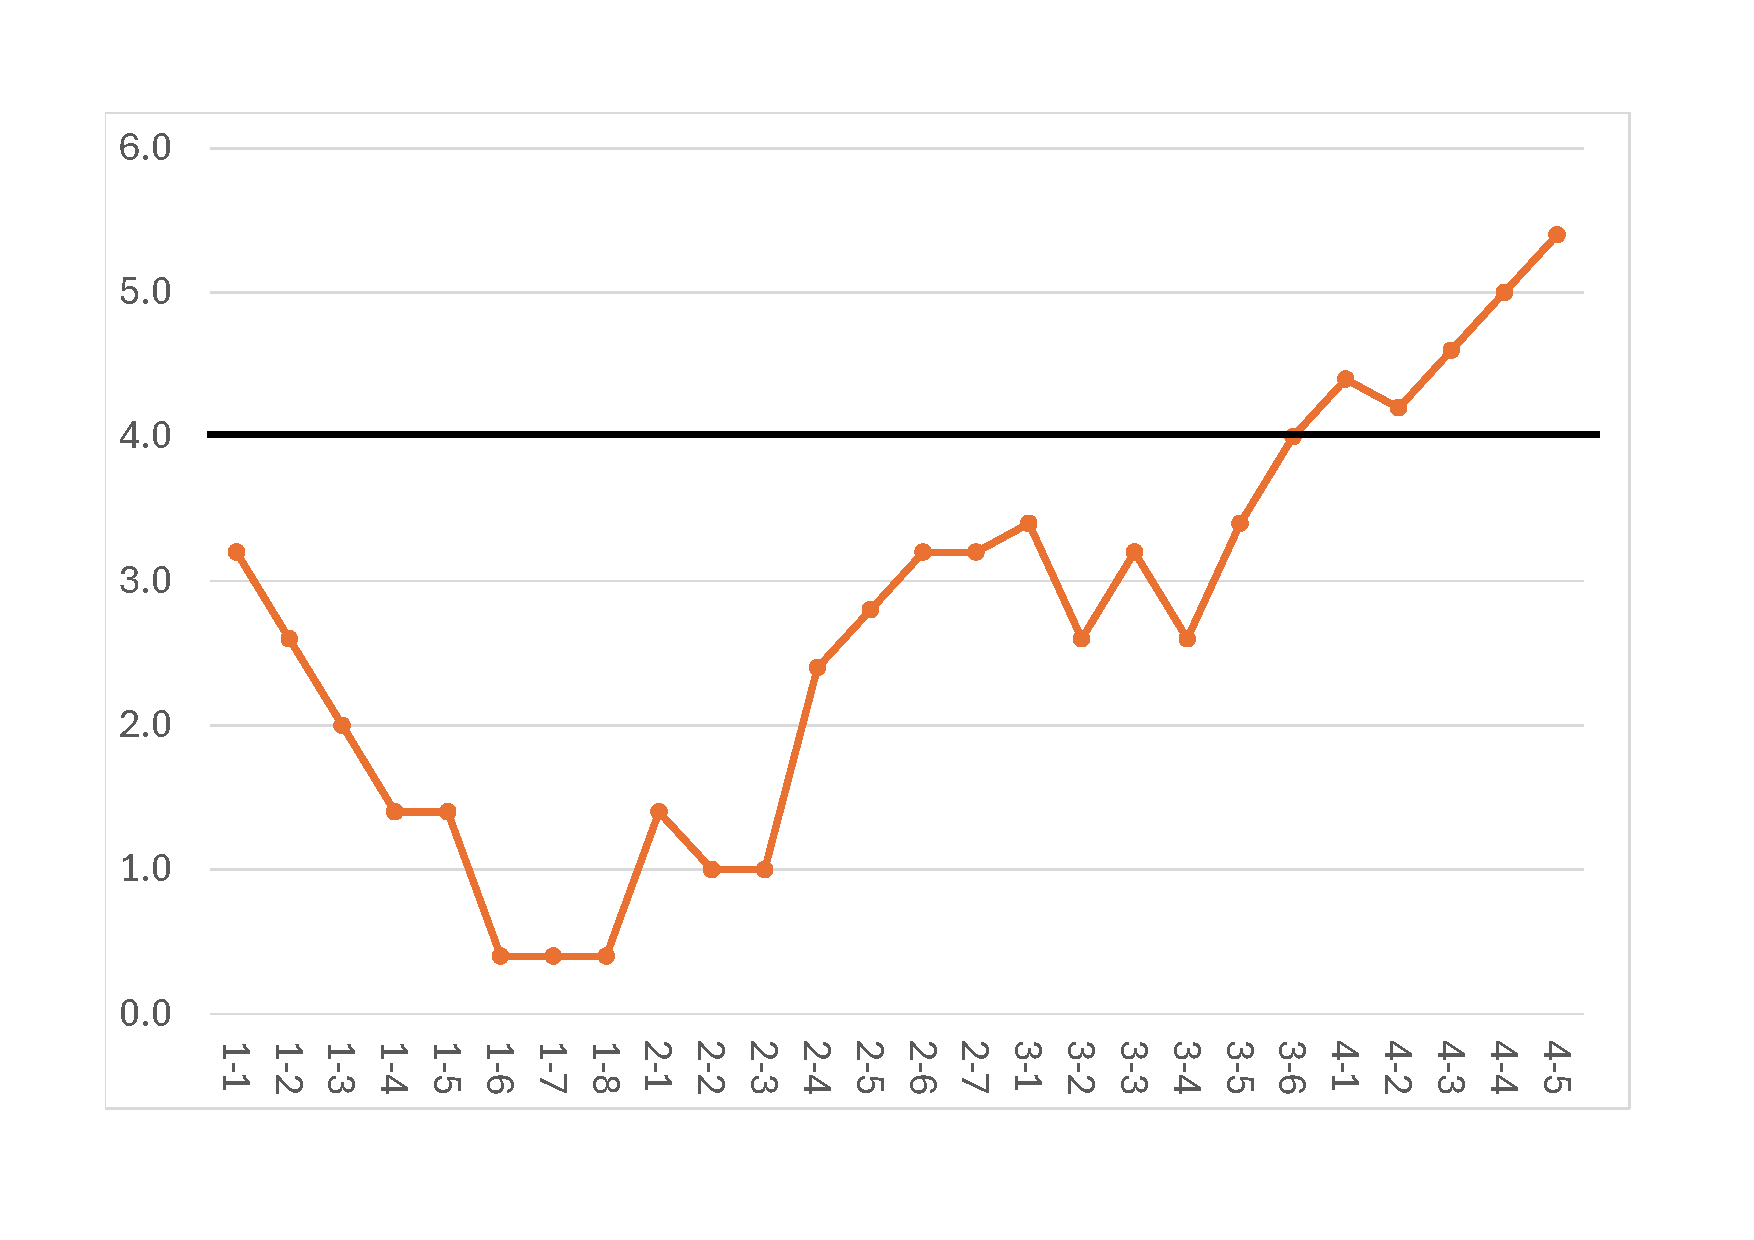
\includegraphics[height=5cm,width=7cm]{2025shinki/wing_span/WS_tokutennkouritu.pdf}
  \caption{ゲーム全体を通じた5ターンごとの得点効率の推移}
  \label{fig:得点効率}
\end{minipage}
\end{figure*}
この図における「絶対必要」と「必要」の違いは、使わなくても(あるいは行動しなくても)済むケースがあるか否かによる。餌コストは(必要ない鳥もあるが、鳥ごとの特徴を無視すれば)鳥をプレイする際には必ず必要になる。一方で卵は各生息地で1回目の発展では必要ない。また、鳥の獲得も1ターンで2枚獲得しておけば、2枚目をプレイする際にはわざわざもう一度鳥カードを獲得する必要はない。この意味で、卵と鳥カードの獲得は「今から鳥をプレイする」となったときに絶対必要だとは限らない。それゆえ、餌の獲得は鳥カードをプレイする上で他の2つよりも優先度が高い。
\par
先ほど述べたように、点数を得るには鳥のプレイと産卵という2通りの方法があった。産む卵の個数を増やすには鳥カードをたくさんプレイすればよい。よって、得点方法はすべて鳥カードのプレイに集約できる。そのうえで、プレイする鳥カードを増やすにはどうすればいいかを考えると、図\ref{fig:発展構造}より最も優先度が高いのは、獲得する餌の量を増やすことであると分かる。すなわち、ゲームが始まったら最初に森林に鳥カードをプレイして、餌の獲得量を増やすべであると言える\footnote{図\ref{fig:発展構造}で「鳥のプレイ」から矢印を逆にたどると「餌の獲得」と「鳥の獲得」がほぼ等価であることが分かる。実際、後で見るように森林の発展と水辺の発展はどちらを先にしても(つまり森林→水辺の順番で発展させても、水辺→森林の順番で発展させても)最終的な点数は理論上あまり変わらない。ただ、私の経験として森林を先に発展させた方が点数が発展するので、本記事では森林の発展の方にウェイトを置いている。なお、ラウンド終了時目的によってはこの限りではない。}。
\end{multicols}
\subsection{理想的な立ち回り}
\begin{multicols}{2}
\subsubsection{得点効率}
2章で述べたことから、ウィングスパンの理想的な立ち回りが導かれる。ただその前に、得点効率という指標について紹介しておく。後で述べる理想的な立ち回りは、この得点効率を最大化するものとして捉えれば理解が深まるからである。
\par
得点効率は以下の式で定義する。
\begin{equation}
  得点効率=\frac{得られる点数}{得点するために使ったターン数}\notag
\end{equation}
要するに1ターン当たり何点得られるかを意味しており、本記事ではゲーム全体を通してこれが最大になるような立ち回りについて論じているのである。
\par
ただこの指標には大域的なものと局所的なものがある。前者は全体を通して得点効率がいくつか、ということだ。例えば80点を取るには全体を通して得点効率が3点ちょっと必要になる。一方後者はある行動をして得点を得る際に、その行動の得点効率はいくつか、ということが問題になる。例えば、鳥カードを引いて、餌を獲得して、鳥カードをプレイする、という一連の流れには原則として3ターンかかる。すると、鳥の得点は高々9点であるから、鳥カードをプレイする操作の得点効率は最大でも3であると言える。いちいち名前を分けるのは面倒くさいので本記事では文脈に応じて意味を使い分けるが、なるべく分かりやすいように書くつもりである。
\par
またここで挙げた例からも分かるとおり、80点をとるには鳥カードをプレイしているだけでは届きそうにない。それゆえ、もっと得点効率の高い(これはどちらかと言えば局所的な意味で)行動をすべきなのである。
\par
実戦において得点効率がどのように推移しているかを見てみよう。図\ref{fig:得点効率}は、私が実際にオートマ戦での操作から5ターンごとの追加点の移動平均を得点効率として割り出して描いたものである。ただし、このグラフではラウンド終了時目的とボーナスカードについては考慮していないことに注意されたい。
\par
グラフの横軸にある数字はラウンドとターンを表している。例えば、1-1は1ラウンド目の1ターン目ということになる。また、最初の2つと最後の2つの値に関しては、端のデータに重きが置かれるように計算した。例えば、1-1の値$a_{1-1}$と1-2の値$a_{1-2}$は$i-j$のデータ$x_{i-j}$を用いて以下の式で表される。
\begin{gather*}
  a_{1-1}=\frac{x_{1-1}+x_{1-1}+x_{1-1}+x_{1-2}+x_{1-3}}{5}\\
  a_{1-2}=\frac{x_{1-1}+x_{1-1}+x_{1-2}+x_{1-3}+x_{1-4}}{5}
\end{gather*}
$a_{4-4}$と$a_{4-5}$も同様である。
\par
このグラフを見て分かるように、局所的な得点効率ははじめは高く、途中に下がったのちに最後にもっとも高くなることが分かる。特に、4ラウンド目には毎ターン4を超えている。この例に限らず、多くのゲームにおいてこの傾向はみられる。この時の最終的な得点は85点であった。鳥をプレイするだけでは得点効率は高々3であったが、最後に得点効率が4を超えたことがプラスに作用したと言えよう。この要因は4ラウンド目のほとんどを産卵に費やしたことである。次節で詳しく述べるが、産卵アクションは最も得点効率が高くなりやすい。それゆえ、4ラウンド目に産卵アクションで回収できる得点ができる限り高くなるように草原に鳥を配置しておくことが肝要なのである。
\subsubsection{理想的な立ち回り}
前節で述べたことを踏まえ、理想的な立ち回りを導く。まず大前提として、得点効率が最も高くなり得るのは産卵である。草原に4枚鳥をプレイしておけばそれだけで1ターンあたり4点は得られるし、それに鳥の能力を加えれば1,2点追加される。運が良ければ1ターンに6点得ることも可能になるのだ。それゆえゲーム全体の目標は4ラウンドに入る前に草原に4枚以上の鳥カードをプレイして、得点するシステムを構築することなのである。
\par
どのようなシステムを構築するかは持っている鳥カードを見て決めるため、草原の開発は最後になる。それまでは森林と水辺を開発することになる。ここでもプレイ時の卵の消費量を考えて3羽プレイすることを目指す。具体的には、まず森林と水辺の両方に2枚鳥をプレイして鳥と餌の供給ラインを作る\footnote{2羽以上プレイすれば、もらえる餌の量や鳥カードの枚数が1つから2つに増える。1ターンで餌が2つ得られれば、2コストの鳥の餌が1ターンでそろうことになる。}。その後、余裕ができたら3枚目をプレイする、という形が理想的である。
\par
以上のようなことを踏まえ、以下のような立ち回りを提唱する。以下、この立ち回りを「理想的な立ち回り」と呼ぶことにする。
\begin{align*}
  &\textbf{1-1} &&森林に鳥カードをプレイ\\
  &\textbf{1-2} &&産卵(2個)\\
  &\textbf{1-3} &&森林に鳥カードをプレイ(卵-1)\\
  &\textbf{1-4} &&鳥カードを獲得(1枚)\\
  &\textbf{1-5} &&餌を獲得(2個)\\
  &\textbf{1-6} &&水辺に鳥カードをプレイ\\
  &\textbf{1-7} &&鳥カードを獲得(1枚)\\
  &\textbf{1-8} &&餌を獲得(2個)\\
  & \tiny{ } && \\
  &\textbf{2-1} &&水辺に鳥カードをプレイ(卵-1)\\
  &\textbf{2-2} &&鳥カードを獲得(2枚)\\
  &\textbf{2-3} &&鳥カードを獲得(2枚)\\
  &\textbf{2-4} &&産卵(2個)\\
  &\textbf{2-5} &&餌を獲得(2個)\\
  &\textbf{2-6} &&草原に鳥カードをプレイ\\
  &\textbf{2-7} &&餌を獲得(2個)\\
  & \tiny{ } && \\
  &\textbf{3-1} &&草原に鳥カードをプレイ(卵-1)\\
  &\textbf{3-2} &&餌を獲得(2個)\\
  &\textbf{3-3} &&草原に鳥カードをプレイ(卵-1)\\
  &\textbf{3-4} &&餌を獲得(2個)\\
  &\textbf{3-5} &&産卵(3個)\\
  &\textbf{3-6} &&草原に鳥カードをプレイ(卵-2)\\
  & \tiny{ } && \\
  &\textbf{4-1} &&産卵(4個)\\
  &\textbf{4-2} &&産卵(4個)\\
  &\textbf{4-3} &&産卵(4個)\\
  &\textbf{4-4} &&産卵(4個)\\
  &\textbf{4-5} &&産卵(4個)\\
\end{align*}
これについてラウンドごとに意味を説明していく。
\par
まず1-1~2-1では、森林と水辺に2枚ずつ鳥カードをプレイするのが目標である。最初に手元に残す鳥を選ぶ段階では鳥の得点や起動時能力よりも餌コストを重視し、開始3ターンで森林に2枚鳥カードをプレイできるようにするのが原則だ。そのために、最初に配られた5枚の鳥カードから手元に残すカードは、必要な餌コストの合計が3で、必要な餌が被っておらず、かつともに森林に生息するような2枚とするのが基本となる。森林を整備した後は水辺の鳥を引き、できるだけ2-1までに水辺にも2枚鳥カードをプレイするようにしたい。また、このフェーズではあまりラウンド終了時目的を取りに行くべきではない。取りに行っても高々4点しか変わらないため、これから先の得点効率を落としてまで取りに行くべきではない。理想的な立ち回り通りにプレイしていたらとれていた、という状況が望ましい。
\par
その後2-2~2-7にかけては草原にプレイする鳥カードを集めるフェーズとなる。できるだけ産卵した時にもう1点取れる鳥カードを集めるようにする。ただ、それだけだとターン数が余ってしまうので、一度鳥をプレイする部分を作ってある。ラウンド終了時目的は取れなさそうなら諦めるべきである。鳥を集める際にボーナスカードの条件も考慮するのは忘れないようにする。
\par
3ラウンド目は、2-2~2-7にかけて集めた鳥をひたすらプレイするフェーズである。ラウンド終了時目的もとれるように鳥を集めておくのがコツである。終了時目的とボーナスカードを絡めるのは少し難しいが、うまくできるとだいぶ得点が安定するようになる。なお、この理想的な立ち回り通りにできない場合は、3ラウンド目の後半に一度時間をとってどうするのが最も得点効率がいいか考えて、それ以降の立ち回りを決めるのを推奨する。終盤になれば、どうするのが最終的にもっとも高得点になるのか計算できるようになるからだ。
\par
最終ラウンドはひたすら産卵するフェーズである。鳥が蓄えられる卵の平均値は2.85個(小数点第3位以下四捨五入)、最頻値は2個(いずれも実際に数えたが、詳細は紙面の都合上割愛)であるから、全体で16~22個程度産卵することができる。このラウンドは最も1ターン当たりの得点効率が高くなる部分であるから、ひたすら産卵を繰り返す。
\par
理想的な立ち回りでは鳥カードで35~40点、ボーナスカードで3~8点、ラウンド終了時目的で10~15点、卵の個数と蓄えた餌の数、差し込んだ鳥カードの枚数をすべて合わせて30~40点の計80~90点程度とれる。もちろん運が良ければ上振れるし、悪ければ80点に届かないこともある。ただ、本記事では以後この立ち回りをモデルケースとして細部を肉付けていきたい。
\subsubsection{例外}
上で述べた理想的な立ち回りはあくまで理想的なもので、様々な仮定の下に実現可能なものである。上の立ち回りができるための条件は、以下の3つである。
\begin{itemize}
  \item 最初に餌コストが1個と2個(しかも被りがない)で森林に生息する2枚の鳥カードがあること
  \item 1-4や1-7で水辺に生息する鳥を引けること
  \item 2ラウンド目で1点稼げる起動時能力を持っており、かつ草原に生息する鳥を引けること
\end{itemize}
これらの条件がそろわない場合は、理想的な立ち回りは実行できない。それゆえ、別途立ち回りのパターンを組む必要がある。上の条件が満たされない場合やパターンでは想定されていないラッキーやアンラッキー(主にアンラッキーの方)を、本記事では「例外」と呼ぶことにする。理想的な立ち回りで生じる例外は、大きく分けて以下の5つだ。
\begin{enumerate}
  \item 最初に4ラウンド目に使える鳥を引いた場合
  \item 最初に森林に生息する鳥を満足に引けなかった場合
  \item 1-4や1-7で水辺に生息する鳥カードが引けなかった場合
  \item 2ラウンド目で1点稼げて草原に生息する鳥カードを引けなかった場合
  \item 2,3ラウンド目で点数の低い鳥カードしか引けなかった場合
\end{enumerate}
これらの例外に対して、次章で対処法を見出していく。紙面の都合上、(i)と(i\hspace{-1.2pt}i\hspace{-1.2pt}i)の2つについてのみ処理する。
\end{multicols}
\subsection{例外処理}
\begin{multicols}{2}
\subsubsection{処理すべき例外と処理しなくてもよい例外}
発生し得る例外をすべて考慮していては途方もなくなってしまう。例えば、最初からずっと草原にしか生息しない鳥カードしか引けないことは理論上あり得るが、起こる確率はとても低い。本記事ではこのような例外に対してもいちいち対処法を考えることはせず、起こったら運の悪さを嘆いて諦める、という立場をとることにする。それゆえ、例外処理に移る前にまず考慮する例外と考慮しない例外について述べておく。
\par
単刀直入に、本記事では発生確率\footnote{ただし、ここでいう発生確率とは条件付き確率のこととは限らないことに注意されたい。条件付き確率を求めている際は、その旨をしっかりと明記している。}が100分の1未満の例外については考慮しない。すなわち、100回に1度も起こり得ないケースが起こった場合は諦める、という立場をとる。例えばある例外を処理していく中で、ここから先のケースは発生確率が100分の1未満だからその手前までで例外は処理されている、というようにして処理を進めていく。このようにしてすべての場合がつくせたら、例外処理完了、ということになる。なお、本記事は全体を通してオートマ戦が基準になっているため、確率計算も次の自分の手番までに鳥カードが1枚も引かれなかったうえでの確率を求めている(これはオートマ戦でも起こることがない、かなり理想的な状況である)。ただ、例外が起こる確率を求める際は、基本的にはカードが引かれていない方が確率が高くなるので、より多くの例外を処理する必要があると考えればそこまで気にする必要はない。

\subsubsection{例外処理(i) 最初に4ラウンド目以降に使える鳥を引いた場合}
この例外は、理想的な立ち回りにおいては2ラウンド目に欲しい鳥が最初に配られた5枚の鳥の中にあった場合を意味している。例えば卵を1個産む起動時能力を持った鳥(そして、このような鳥はたいてい草原にしか生息しない)が最初に配られたカードにあった場合などがこれにあたる。結論から言えば、森林か水辺に生息していない限りそのようなカードは最初に捨ててもよい。なぜならば、起動時能力で1点稼げる鳥カードは2ラウンド目に引けばよいのであって、最初に引けたからといってそこに執着していては餌や鳥カードの供給ラインを整備することもままならなくなり、本末転倒だからである。最初に意識すべきは森林と水辺に2枚ずつ鳥カードをプレイすることであって、起動時能力で1点稼げる鳥を引くことではない。捨てるのはもったいないかもしれないが、またあとで巡り合えると信じて一旦手放すのが最善手になる。ただ、森林や水辺に生息する鳥カードが引けなかった場合や引けても1枚程度だった場合はその限りではない。その場合は例外(i\hspace{-1.2pt}i)に相当するが、これについては本記事では扱わない。
\subsubsection{例外処理(i\hspace{-1.2pt}i\hspace{-1.2pt}i) 1-4や1-7で水辺に生息する鳥カードが引けなかった場合}
まずはこの例外が発生する確率を求める。前提としてこの例外は初めに配られた鳥カードに森林に生息する鳥が十分にあった場合に発生するものであるから、欲しいのはそのうえで水辺に生息する鳥カードを引けない条件付き確率である。さらに、その条件付確率が最も大きくなるのは、初めに水辺に生息する鳥カードのみを引いたときである。よって、水辺に生息する鳥カードは計85枚あるので、この例外が起こる条件付き確率は最大で
\begin{equation*}
  \frac{{}_{85} \mathrm{C}_3}{{}_{165} \mathrm{C}_3}\times\frac{82}{162}\times\frac{81}{161}=0.0342\cdots>0.01
\end{equation*}
となる。よってこの例外が発生する確率は高々0.034(30回に1回程度)と言える。低いが、0.01を超えてはいるので、一応処理を検討しておく。一方で上の状態からもう1回カードを引いても水辺に住む鳥を引けない確率は、
\begin{equation*}
  \frac{{}_{85} \mathrm{C}_3}{{}_{165} \mathrm{C}_3}\times\frac{82}{162}\times\frac{81}{161}\times\frac{80}{160}=0.0171\cdots>0.01
\end{equation*}
であり、ここからもう1回カードを引くと、水辺に住む鳥カードが得られない確率が0.01を下回る。よって、3回鳥カードを引いても水辺に住む鳥を獲得できない場合に対して処理を与えればよい。
\par
理想的な立ち回りにおいて、1-4以降3回鳥カードを引いても水辺に住む鳥を引けなかったという体で、それ以降の立ち回りを組む。1例として、以下のような立ち回りを提唱する。

\begin{align*}
  &\textbf{1-1} &&森林に鳥カードをプレイ\\
  &\textbf{1-2} &&産卵(2個)\\
  &\textbf{1-3} &&森林に鳥カードをプレイ(卵-1)\\
  &\textbf{1-4} &&鳥カードを獲得(1枚)\\
  &\textbf{1-5} &&餌を獲得(2個)\\
  &\textbf{1-6} &&草原に鳥カードをプレイ\\
  &\textbf{1-7} &&鳥カードを獲得(1枚)\\
  &\textbf{1-8} &&餌を獲得(2個)\\
  & \tiny{ } && \\
  \displaybreak
  &\textbf{2-1} &&草原に鳥カードをプレイ(卵-1)\\
  &\textbf{2-2} &&鳥カードを獲得(1枚)\\
  &\textbf{2-3} &&餌を獲得(2個)\\
  &\textbf{2-4} &&産卵(3個)\\
  &\textbf{2-5} &&草原に鳥カードをプレイ(卵-1)\\
  &\textbf{2-6} &&鳥カードを獲得(1枚)\\
  &\textbf{2-7} &&餌を獲得(2個)\\
  & \tiny{ } && \\
  &\textbf{3-1} &&草原に鳥カードをプレイ(卵-2)\\
  &\textbf{3-2} &&鳥カードを獲得(1枚)\\
  &\textbf{3-3} &&餌を獲得(2個)\\
  &\textbf{3-4} &&水辺に鳥カードをプレイ\\
  &\textbf{3-5} &&鳥カードを獲得(1枚)\\
  &\textbf{3-6} &&餌を獲得(2個)\\
  & \tiny{ } && \\
  &\textbf{4-1} &&産卵(4個)\\
  &\textbf{4-2} &&水辺に鳥カードをプレイ(卵-1)\\
  &\textbf{4-3} &&産卵(4個)\\
  &\textbf{4-4} &&産卵(4個)\\
  &\textbf{4-5} &&産卵(4個)\\
\end{align*}
これについても順を追って説明する。
\par
まず1-3までは理想的な立ち回り通りである。1-4以降は、水辺に生息する鳥カードが得られないので、草原に住む鳥カードを引く\footnote{この時に鳥の山から引いて森林にしか生息しない鳥カードを引いても後の立ち回りはさほど変わらない。草原の列にプレイされている鳥カードが1枚減って、森林の列にプレイされている鳥カードが1枚増えるだけである。この場合は産む卵が少なくなる分70点ぐらいが標準だと思われる。}。しばらく「草原にすむ鳥カードを引く→餌を獲得→(必要なら産卵→)鳥カードのプレイ」という流れを繰り返し、草原に4枚の鳥カードをプレイしておく。そうすると、1回で4個の卵を産めるようになる。それから3ラウンド終了までの余ったターンは、森林か水辺にすむ鳥カードを引き、順にプレイしていって鳥カードの点数を稼ぐ。最後の4ラウンド目では、3-5で引いた鳥カードを途中でプレイするほかは毎ターン4個ずつ卵を産んでいって得点を稼ぐ。
\par
この立ち回りでは鳥カードの得点32点、ボーナスカード3,4点、ラウンド終了時目的10点、卵15個、蓄えた餌の個数と差し込んだ鳥カードの点数が合わせて10点の合計70点程度が期待できる。もちろん早い段階で卵を産む起動時能力を持った鳥をプレイできれば、4-1でもう1羽鳥をプレイしてもう少し点数を伸ばすこともできる。ギリギリ80点には届いていないが、ここまで起こり得ないアンラッキーな例外で70点取れるなら上出来だろう。
\par
この立ち回りの肝は、プレイする鳥カードの枚数を増やせない分を、産む卵の個数を増やすことで補填するという点である。そのために草原に4枚以上の鳥カードをプレイすることが望ましい。ただ、基本的には多くの鳥カードを引けなければプレイの選択肢が狭まり、鳥の得点はおろかボーナスカードや終了時目的での得点も難しくなるので、80点をとるのはなかなか厳しい\footnote{この点を考慮すると最初に発展させるのは水辺の方がいいような気もしてくるが、うまく水辺に鳥カードをプレイできたとしても、多くの場合餌がなかなかそろわないのでなかなかゲームが進まない。最初の2ターンで森林と水辺に1枚ずつプレイしておくというのもアリだが、それも餌ガチャと鳥カードガチャの両方に足を突っ込むことになり、微妙な気もする。}。
\par
以上で例外(i\hspace{-1.2pt}i\hspace{-1.2pt}i)は解決された。
\end{multicols}
\subsection{おわりに}
\begin{multicols}{2}
本記事では、最初にウィングスパンのルール分析から発展構造を図におこし、それを用いて理想的な立ち回りを導いた。ただこの立ち回りはあくまで理想的なものであって、様々な都合の良い仮定のもとに成り立っている。そこで、そうした仮定が成り立たない場合を例外として列挙し、対処法を模索した。具体的には、発生確率が0.01未満のものに関しては考慮すべきものではないとして切り捨て、それ以外のものに対しては、理想的な立ち回りと比べて得点効率が下がり得るのか検討した。下がり得ないものは理想的な立ち回りを柔軟に変えて対処し、下がり得るものは、そのケースでも80点近くとれるような代替の立ち回りを提唱した。
\par
本記事を通してウィングスパンの定石というものがある程度確認されたのではないかと私は考えている。まず1ラウンド目で森林と水辺に2枚の鳥カードをプレイし、2ラウンド目で草原にプレイする鳥カードを収集し、3ラウンド目にそれらの鳥カードをプレイし、最後の4ラウンド目でひたすら産卵して得点を稼ぐ、という、安定して点数を得るための機械的な立ち回りが一つ得られた。実践では、これをもとにボーナスカードやラウンド終了時目的を考慮して臨機応変に対応すればよい。想定していなかった例外が発生しても、できる限りどこかで理想的な立ち回りと合流できるような手を打っていけばいい。
\par
また、定石を導いたのみならず、導き方のアウトラインを与えたことも、本記事における成果の一つである。ウィングスパンのような発展構造がループしているボードゲームに関しては、その構造を整理すれば、一番最初に手を付けるべきところが定まる。そこからゲームの得点しどころを見極め、そこでの得点効率を最大化するように手順を整備すれば、それが一つの定石になるというわけである。本記事で私がとった手法を応用していけば、似たような性質を持つ他のゲームについても容易に定石を構築できるようになるはずである。
\par
一方で、本記事では解決できなかったこともいくつかある。まず挙げられるのは、拡張版で遊ぶ際にはどうすればいいか、という問いである。本記事で扱ったのは無印のウィングスパンであるが、2024年現在、ウィングスパンには他にも欧州、大洋、東洋、という3つの拡張版があり、これらには新しい鳥に加え、無印にはなかった終了時目的、能力などが加わり、よりゲームを複雑にしている。それらについても今後分析していく必要がある。また、より細かい点を挙げれば、私はまだ以下のことが分かっていない。
\begin{itemize}
  \item ボーナスカードやラウンド終了時目的の活かし方
  \item 鳥の能力の詳細な分類と、能力の活用法
  \item 常に最善手を打った際にとり得る点数の分布
  \item 対人戦におけるインタラクションについて\footnote{まぁ一緒に研究してくれる人がいないので調べられないのだが。}
\end{itemize}
こうしたことはウィングスパンを完全に理解するためには知っておく必要があるため、今後の研究で取り組むべき課題であろう。本記事をきっかけにして、ウィングスパンはもちろんのことより多くのボドゲの定石研究が盛んになれば、それは筆舌に尽くしがたい幸福である。
\par
ここまで非常に長くなったが、最後に。私がウィングスパンを研究し始めた当初は、鳥カードは餌コストと得点、産む卵の個数、能力を対応させる記号にしか見えなかった。きっかけとなった耐久ボドゲ会でも、他の2人が鳥カードを愛でているそばで「かわいいのは分からなくはないんだけどなあ...」と、いまいち腑に落ちない気持ちであった。しかし、研究のためにオートマ戦を繰り返す中で、ふと鳥カードをかわいいと思う瞬間があった。その時を境に私は遊びながら鳥を愛でることを覚え、かくして2人、そしてウィングスパンを遊ぶ他の談話室民たちの仲間入りをしたのである。
\par
私の推しは「アオバネアメリカムシクイ」、「クロズキンアメリカムシクイ」、「オウゴンアメリカムシクイ」、「ミズイロアメリカムシクイ」の4羽である。
\end{multicols}
\begin{figure}[h]
\centering
\begin{minipage}[b]{0.23\columnwidth}
    \centering
    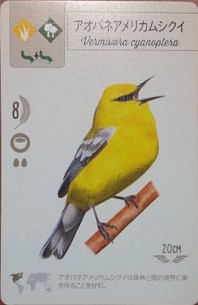
\includegraphics[width=0.9\columnwidth]{2025shinki/wing_span/aobaneamerikamusikui.jpg}
    \caption{アオバネアメリカムシクイ}
    \label{fig:アオバネアメリカムシクイ}
\end{minipage}
\begin{minipage}[b]{0.23\columnwidth}
    \centering
    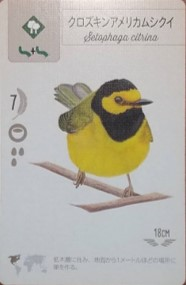
\includegraphics[width=0.9\columnwidth]{2025shinki/wing_span/kurozukinnamerikamusikui.jpg}
    \caption{クロズキンアメリカムシクイ}
    \label{fig:クロズキンアメリカムシクイ}
\end{minipage}
\begin{minipage}[b]{0.23\columnwidth}
    \centering
    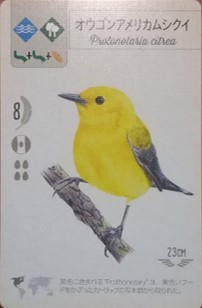
\includegraphics[width=0.9\columnwidth]{2025shinki/wing_span/ougonamerikamusikui.jpg}
    \caption{オウゴンアメリカムシクイ}
    \label{fig:オウゴンアメリカムシクイ}
\end{minipage}
\begin{minipage}[b]{0.23\columnwidth}
  \centering
  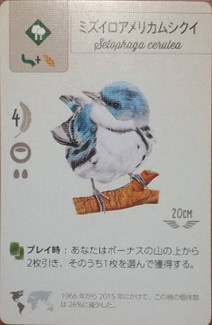
\includegraphics[width=0.9\columnwidth]{2025shinki/wing_span/mizuiroamerikamusikui.jpg}
  \caption{ミズイロアメリカムシクイ}
  \label{fig:ミズイロアメリカムシクイ}
\end{minipage}
\end{figure}
\begin{multicols}{2}
\par
やはり何と言っても絵柄がかわいい。ぬいぐるみにしたらやや小太りでふさふさの毛並みをしていそうで愛くるしい。抱きかかえて頭をなでなでしたくなる。しかも鳥効率が高いものばかりで強いところもいいし、翼長が短いのでハヤブサなどの起動時能力で引いたときも残念な気分にならない。それどころか、少し可哀そうな気分にさえなる。なにせ捕食者の能力で食べられちゃうので。
\par
推し鳥ができてから、私のウィングスパンは格段に幸せなものになった。カードを引いてゲットできたらうれしくなるし、鳥の山から3枚とって公開した時に見えた際にはすぐに取りに行く(実際強いから別に悪手ではない)。相手にとられると悲しくもなる。こんなかわいい鳥たちがいるウィングスパンを買ってきてくれた現&元談話室民には非常に感謝しているし、私が廃れるきっかけを作ってくれた同期のボドゲ民たちには頭が上がらない。
\end{multicols}